\chapter{Introdução}
\label{cap:introducao}

Os sistemas de transporte se estabeleceram ao longo da história como um dos principais condicionantes ao desenvolvimento humano. Em sua utilização, seja para circulação de pessoas ou escoamento de produção, intensifica-se cada vez mais demandas por eficiência, dado seu fator estratégico. Neste contexto, com o avanço das tecnologias computacionais, surgiram os Sistemas de Transporte Inteligentes (\textit{Intelligent Transport Systems} - ITS), os quais constituem soluções tecnológicas desenvolvidas para aprimorar o desempenho e a segurança dos sistemas de transporte \cite{Zhang2011,Aragon2016}. Nestas aplicações, o ambiente de tráfego é monitorado através de sensores empregados na infraestrutura de transporte e seus participantes \cite{Zhang2011,mathew2014a,mathew2014b}. Estes sensores produzem dados brutos que são posteriormente processados por modelos computacionais para gerar informações situacionais acerca do modal \cite{Zhang2011}.

Os dados situacionais produzidos em ITS podem ser classificados de diversas maneiras. Uma delas, a percepção veicular, os sensores são empregados de forma a ser possível produzir exterocepções e propriocepções \cite{menegazzo2020}. A exterocepção busca compreender o ambiente fora do veículo, realizando o reconhecimento de características do caminho no qual trafega. Estas características incluem eventos transientes, sendo anomalias e obstáculos tais como buracos, trincas em malha, lombadas etc.; e persistentes, como tipo de pavimentação, condição de conservação e qualidade da superfície da pista. A propriocepção, por sua vez, objetiva compreender os movimentos veiculares para identificar seu próprio comportamento. Estas identificações também podem ser transientes, como eventos de condução, do tipo troca de pista, frenagem, derrapagem, aquaplanagem, virando à direita ou esquerda; e persistentes, como perfil de comportamento de condução em seguro ou perigoso \cite{menegazzo2018,menegazzo2020}.

As informações situacionais produzidas possuem grande aplicabilidade, com impactos sociais, econômicos e ambientais. No suporte à tomada de decisão humana, dados como qualidade do pavimento, e geolocalização de obstáculos e irregularidades na pista podem ser empregados em sistemas gerenciais para planejamento de rotas no escoamento de produção, uma vez que o inadequado estado de conservação do pavimento produz, em média, elevação de 27,0\% dos custos operacionais \cite{CNT2017}. Estes dados também podem ser utilizados por administradoras da via para planejamento de manutenções e controle de tráfego, ou por usuários em Sistemas Avançados de Assistência ao Motorista (\textit{Advanced Driver-Assistance Systems} - ADAS), melhorando a segurança no trânsito. No suporte à tomada de decisão artificial, além dos dados supracitados, outros como tipo de pavimento e perfil de condução podem ser utilizados em veículos autônomos para auxiliar na coordenação de suas ações.

Para a produção dos dados brutos que, após processados, geram as informações na forma de percepção veicular, tecnologias com diferentes abordagens foram propostas, dentre métodos intrusivos e não-intrusivos \cite{NI2016}, conforme ilustra a \autoref{fig:classificacao_sensores}. Na abordagem intrusiva, os dados brutos são amostrados através de sensores colocados diretamente na superfície de via, requerendo possíveis alterações no pavimento ou no tráfego \cite{mathew2014a}. Já na abordagem não-intrusiva, não são realizadas alterações na infraestrutura da via, com os sensores colocados dentro dos veículos que nela trafegam \cite{mathew2014b}. Os métodos não-intrusivos possuem diversas vantagens em relação aos intrusivos, tais como serem menos onerosos, de fácil instalação, cobrirem uma área de monitoramento muito maior e permitirem, além da inspeção da infraestrutura, o acompanhamento das ações dos participantes através da propriocepção.

\begin{figure}[h]
  \centering
  \caption{Abordagens de sensoriamento em ITS}
  \label{fig:classificacao_sensores}
  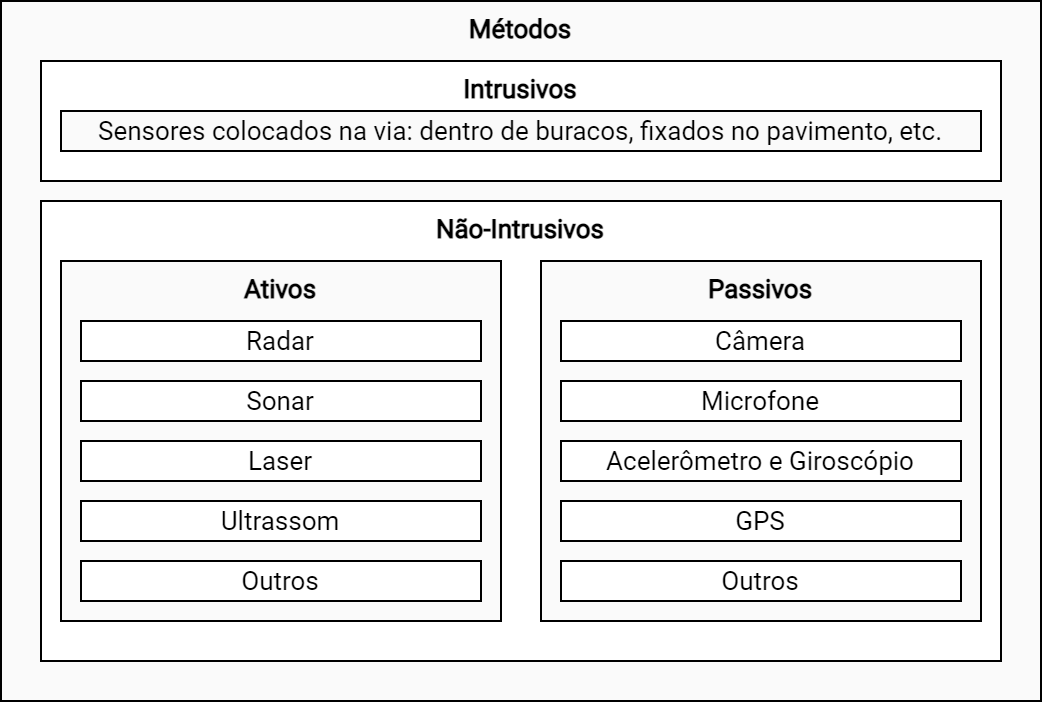
\includegraphics[width=0.9\linewidth]{figuras/fig_1.png}
  \fonte{Desenvolvido pelo autor.}
\end{figure}

Na abordagem não-intrusiva, são empregadas técnicas de sensoriamento passivo e ativo. As técnicas ativas requerem interação com o ambiente para produzir seus dados brutos, com a emissão de ondas no ambiente externo através de laser, ultrassom, sonar ou radar. As técnicas passivas, por sua vez, amostram seus dados sem necessitar interagir com o ambiente externo, como dados físicos ou imagens. Em comparação ao sensoriamento ativo, a abordagem passiva é considerada mais segura, não poluente e geralmente de menor custo. Essas características tornam estas técnicas mais interessantes para uso em larga escala, tal como sua aplicação em sistemas tipo do ADAS ou veículos autônomos. Dentre as soluções de sensoriamento passivo, a utilização de câmeras tem sido amplamente explorada nos últimos anos, com o desenvolvimento de soluções robustas em visão computacional. Contudo, o mesmo não ocorre com os sensores inerciais, representados por acelerômetro e giroscópio, os quais constituem uma alternativa importante a ser melhor explorada \cite{menegazzo2018,menegazzo2020}.

\section{Contextualização do Problema}

Classificados como não-intrusivos e passivos, os sensores inerciais se baseiam no princípio da inércia para produção de seus dados \cite{Braga2017}. Representados por giroscópios e acelerômetros, estes dispositivos produzem, respectivamente, sinais unidimensionais referentes a taxa de rotação e a força de aceleração em seus três eixos físicos \cite{Groves2013}. Neste estudo, estes sinais são resultantes da tração do veículo e das interações com o ambiente no qual ele trafega. Através da aplicação em veículos, sejam fixados diretamente na estrutura veicular ou embarcados em dispositivos móveis como \textit{smartphones} e \textit{tablets}, os sensores inerciais permitem a produção de uma grande diversidade de informações situacionais, conforme ilustra a \autoref{fig:percepcoes_veiculares}.

\begin{figure}[h]
  \centering
  \caption{Percepções veiculares produzidas através de dados de sensores inerciais}
  \label{fig:percepcoes_veiculares}
  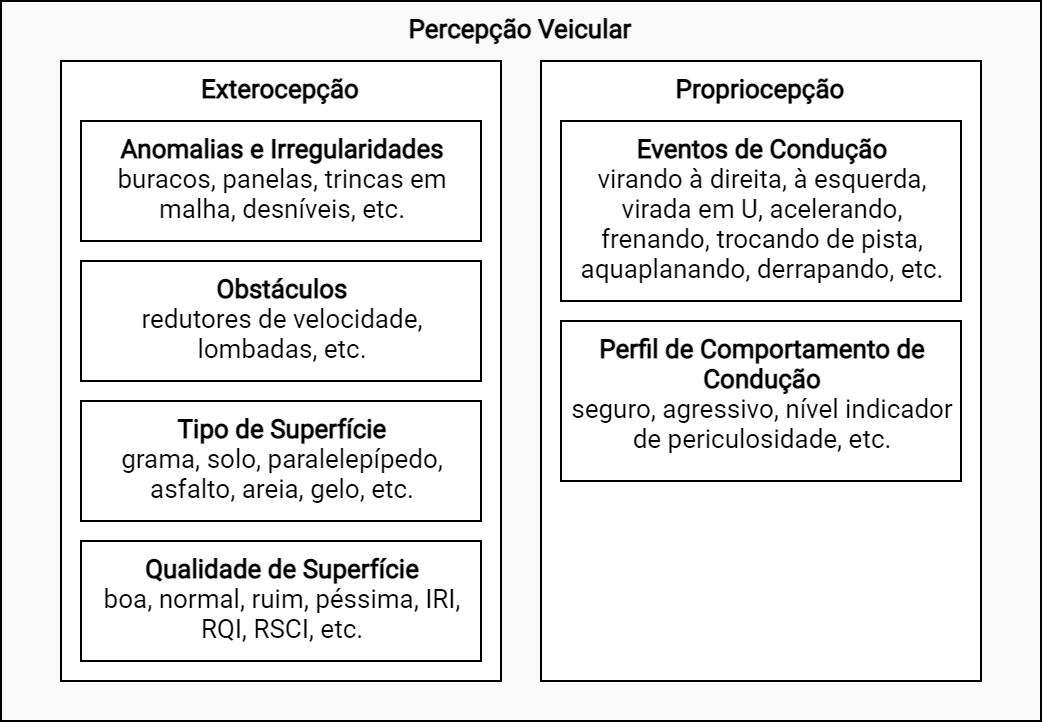
\includegraphics[width=0.9\linewidth]{figuras/fig_2.png}
  \fonte{Desenvolvido pelo autor.}
\end{figure}

Embora sejam diversas e relevantes as percepções veiculares produzidas, a utilização de sensores inerciais em ITS pouco avançou nos últimos anos. Através da Revisão Sistemática da Literatura (RSL) \cite{menegazzo2018,menegazzo2020}, foi observado que a maioria dos estudos da área apresenta foco na aplicação das percepções produzidas. Sendo assim, consistem em pesquisas na forma de prova de conceito, onde as soluções apresentadas para produção de percepções veiculares são simplistas e não aplicáveis a cenários do mundo real, devido a inadaptabilidade dos modelos. Contudo, entendemos que a adaptabilidade é um recurso essencial, onde a solução desenvolvida precisa apresentar um certo grau de confiabilidade quando aplicada em cenários não controlados onde há variações contextuais. Em uma análise comparativa, enquanto soluções baseadas em imagens/vídeos se mostram maduras, com análises em variações contextuais tais como avaliação em diferentes dimensões, marcações desbotadas, diferentes condições de iluminação e oclusão por causa de veículos ou pedestres \cite{Srimongkon2017, Patil2020}, o mesmo não ocorre com os modelos baseados em sinais de sensores inerciais. Nas aplicações desenvolvidas com estes sensores, os modelos analisam cenários controlados e limitados, sem considerar variações de condições no contexto que influenciam os sinais amostrados e, portanto, o resultado da solução final \cite{menegazzo2018,menegazzo2020}.

De acordo com \cite{Carlos2019}, nos últimos 10 anos se produziu uma literatura vasta sobre modelos para produzir informações situacionais a partir dos dados de sensores inerciais fixados no veículo ou embarcados nos \textit{smartphones}. Contudo, é necessário em novas pesquisas tornar os modelos mais inteligentes para traçar o perfil das estradas com detalhes reais \cite{Carlos2019}. Esta afirmação também é sustentada pelos resultados obtidos no levantamento do estado da arte \cite{menegazzo2018,menegazzo2020}, onde observa-se que para um modelo de percepção veicular operar de forma segura e confiável em cenários do mundo real, é necessário considerar os fatores de dependência que impactam nos sinais dos sensores inerciais. Estes fatores estão relacionados à diversidade contextual existente, onde o modelo pode ser aplicado a diferentes veículos, motoristas e ambientes. Considerar estes fatores no modelo o torna adaptável a diferentes condições, sendo este um requisito essencial para sua ampla utilização.

\section{Objetivos}

Nesta seção são detalhados o objetivo geral e específicos desta pesquisa.

\subsection{Objetivo Geral}

Este trabalho objetiva desenvolver modelos adaptativos para produção de percepções veiculares com emprego de sinais de sensores inerciais e técnicas de Inteligência Artificial (IA).  Para satisfazer o requisito de adaptabilidade, os modelos devem demonstrar boa capacidade de generalizar seu aprendizado quando submetido a contextos desconhecidos, os quais apresentam variações contextuais relacionadas as suas propriedades de dependência.

\subsection{Objetivos Específicos}

Os objetivos específicos deste trabalho são:

\begin{itemize}

\item Identificar o estado da arte acerca da produção de percepção veicular através de sinais de sensores inerciais;

\item Desenvolver uma infraestrutura e uma metodologia para coleta de dados brutos;

\item Produzir conjuntos de dados com variações contextuais das propriedades de dependência;

\item Desenvolver um modelo para classificação do tipo de superfície de pista, classificando os sinais dos sensores inerciais entre segmentos de terra, paralelepípedo ou asfalto;

\item Desenvolver um modelo para classificação da irregularidade de superfície de pista,  classificando os sinais dos sensores inerciais entre segmentos de qualidade ruim, regular ou boa;

\item Desenvolver um modelo para detecção de lombadas, através de sinais dos sensores inerciais;

\item Validar a adaptabilidade dos modelos através de um \textit{design} experimental, onde cada modelo será avaliado quanto a sua capacidade de generalização de aprendizado para contextos desconhecidos;

\end{itemize}

\section{Justificativa}

Para disseminar a utilização de ITS em suas mais variadas formas, mostra-se necessário tornar estes sistemas cada vez mais inteligentes. Para isto, é necessário dispor de mais fontes de dados, que estes dados sejam confiáveis, e que os dispositivos que os produzem não sejam prejudiciais à saúde humana quando aplicados em massa. Sendo assim, os sensores inerciais constituem uma fonte de dados alternativa, com grande potencial de melhorar as aplicações em ITS. Devido a sua abordagem passiva, se mostra um meio seguro, não poluente e de baixo custo. A segurança de sua aplicação em massa já foi amplamente validada, uma vez que todo \textit{smartphone} e \textit{tablet} possui um conjunto destes dispositivos. Os sinais produzidos pelos sensores permitem a produção de uma grande variedade de percepções veiculares, dentre exterocepções e propriocepções. Contudo, os atuais modelos de percepção veiculares baseados em sensores inerciais não são confiáveis, se mostrando o principal entrave para sua maior adoção.

A não confiabilidade nos modelos atuais se deve essencialmente a falta de adaptabilidade das soluções. Desta forma, os modelos desenvolvidos não mantêm sua efetividade quando aplicados em cenários diferentes do qual foi experimentado. Sendo assim, os estudos no estado da arte não consideram as variações contextuais pelas quais o modelo será submetido, e os fatores de dependência relacionados. Desta forma, o desenvolvimento de um modelo adaptativo de percepção se mostra de grande contribuição, seja aplicada na tomada de decisão humana ou artificial. Constituindo um aplicação meio para outros sistemas, diversas áreas dos ITS podem se beneficiar, como veículos autônomos, Sistemas Avançados de Controle de Veículos (\textit{Advanced Vehicle Control Systems} - AVCS), Sistemas Avançados de Informação ao Viajante (\textit{Advanced Traveler Information Systems} - ATIS), Sistemas Avançados de Gerenciamento de Tráfego (\textit{Advanced Traffic Management Systems} - ATMS), Sistemas Avançados de Gerenciamento de Transporte Público (\textit{Advanced Public Transport Management Systems} - APTMS), ADAS, entre outros \cite{Zhang2011,Singh2015}.

\subsection{Cenários de Aplicação}

Nesta seção são detalhados alguns cenários de aplicação dos modelos propostos.

\begin{description}

\item [Veículos Autônomo:] Um veículo equipado com sensores inerciais e auxiliares de suporte trafega em uma via. A irregularidade longitudinal da pista, correspondente ao conjunto dos desvios da superfície, é processada em relação a um plano de referência. Nesta análise, é estabelecido um índice de qualidade de conservação e identificado o tipo de pavimentação da via. Também são reconhecidos e classificados eventos transientes de percepção de ambiente, como obstáculos na via (lombadas, redutores de velocidade etc.), deficiências da superfície (buracos, solavancos etc.); e de propriocepção, como eventos de condução (virando à direita suave ou bruscamente, virando à esquerda, acelerando, frenando etc.). Disponibilizando estas informações através de uma interface ao agente inteligente que controla o veículo, o índice de qualidade de superfície e o tipo de pavimentação aferido são empregados no controle de velocidade veicular, sendo menor em vias mais irregulares e vice-versa. Esta decisão pode ser monitorada através dos eventos de condução e, se necessário, efetuado ajustes de comando. Os eventos transientes detectados de percepção de ambiente, utilizados na forma de evidências, auxiliam na convalidação de dados obtidos de sensores multimodais, tal qual por intermédio de visão computacional, corroborando hipóteses sobre o contexto no qual está inserido.

\item [Sistema Avançado de Assistência ao Motorista:] Em um sistema de \textit{vehicular crowdsensing} com sensoriamento oportunista, um \textit{crowdsourcer} utiliza um aplicativo de ADAS em seu computador de bordo ou \textit{smartphone}. Com os sensores inerciais anexados ao veículo ou embarcados nos dispositivos móveis, o aplicativo analisa as vibrações recebidas, para estabelecer conceitos qualitativos sobre a irregularidade de superfície e reconhecer eventos transientes, na forma de obstáculos e anomalias. Um servidor central recebe dados de vários \textit{crowdsourcers}, onde aplica-se um aprendizado baseado em reforço. Empregando a confiabilidade inicialmente estabelecida e a quantidade de detecções em diferentes fontes, a aplicação central realiza ajustes periódicos dos valores de confiabilidade dos dados, de forma que falsos positivos tenham progressivamente sua confiabilidade reduzida a zero, assim como algum evento transiente que deixe de existir, especialmente em função das manutenções realizadas na via. Com esse processamento no servidor, os dados atualizados são baixados pelos \textit{crowdsourcers}, de forma que o aplicativo ADAS utiliza-os para auxiliar o motorista, alertando-o sobre a velocidade acima da segura para uma pista com aquela qualidade de superfície, obstáculos e deficiências durante o trajeto.

\item [Sistema de Monitoramento de Infraestrutura de Transporte Terrestre:] Um veículo e\-qui\-pa\-do com sensores inerciais e auxiliares de suporte trafega em uma via. A irregularidade longitudinal da pista, correspondente ao conjunto dos desvios da superfície, é processada em relação a um plano de referência. Nesta análise, é estabelecido um índice de qualidade de conservação e identificado o tipo de pavimentação da via. Também são reconhecidos e classificados eventos transientes de percepção de ambiente, como obstáculos na via (lombadas, redutores de velocidade etc.), deficiências da superfície (buracos, solavancos etc.). Estas informações situacionais são salvas em um servidor remoto, com as respectivas coordenadas geodésicas. Posteriormente, estes dados são utilizados para definir a manutenção das vias, quando e onde deve ocorrer. Estes dados podem integrar relatórios governamentais, tais como o Relatório Gerencial produzido pela Confederação Nacional do Transporte (CNT), de forma a auxiliar direcionamento de investimentos públicos no modal de transporte terrestre.

\end{description}

\section{Contribuições}

Este trabalho apresenta diversas contribuições de aspecto teórico e aplicado. Com a produção de uma ampla revisão sistemática da literatura, foi realizado o levantamento do estado da arte na aplicação de sensores inerciais para produção de percepções veiculares. Através da análise deste levantamento, foram mapeados todos os fatores de dependência existentes no contexto de ITS que influenciam os sinais amostrados através de sensores inerciais. Este mapeamento, até então inexistente, é importante para que se possa desenvolver modelos de percepção veicular mais robustos, com adaptabilidade ao contexto. Junto a estes fatores, foram produzidos mapeamentos de aspectos diversos, que compreendem desde a etapa da coleta de dados, pré-processamento e processamento.

Com o estabelecimento do estado da arte e mapeamento de aspectos importantes nesta área de pesquisa, foi desenvolvida uma metodologia de coleta de dados, a qual compreende desde a criação da rede de sensores, referenciais de coleta e análise, colocação e posicionamento dos sensores na infraestrutura veicular, etc. Através dessa metodologia, foram produzidos nove conjuntos de dados com variações contextuais relacionadas aos fatores de dependência: diferentes veículos, motoristas e ambientes. Baseando-se nos conjuntos de dados, produzimos um \textit{design} experimental compreendendo as etapas de treinamento e validação dos modelos, de forma a ser possível avaliar a eficiência da generalização de aprendizado do modelo quando aplicado a um contexto desconhecido. Por fim, através de técnicas de \textit{Deep Learning} foram desenvolvidos três modelos adaptativos de percepção veicular, de forma que suas camadas de processamento fossem capazes de compreender as relações entre os dados e seus fatores de dependência. O primeiro modelo classifica o tipo de superfície de pista. O segundo, a qualidade da superfície. Por fim, o terceiro identifica lombadas na via.

Este projeto é inteiramente \textit{open-source}, disponibilizado no Github \footnote{https://github.com/Intelligent-Vehicle-Perception/Intelligent-Vehicle-Perception-Based-on-Inertial-Sensing-and-Artificial-Intelligence} \footnote{https://codigos.ufsc.br/lapix/intelligent-vehicle-perception-based-on-inertial-sensing}. Desta forma, os códigos-fonte utilizados na coleta de dados, para manipulação de sensores, amostragem e armazenamento dos sinais; no pré-processamento, com ajustes, combinação de dados, normalização, etc.; no processamento, com a classificação dos padrões; assim como os próprios datasets e modelos desenvolvidos, estão documentados e disponíveis publicamente, permitindo pesquisas futuras executarem, compararem e auditarem os experimentos. Convém mencionar que os conjuntos de dados produzidos são provavelmente os primeiros do tipo a serem disponibilizados publicamente, com coleta em múltiplos pontos e emprego de diversos sensores de abordagem passiva. Adicionalmente, o projeto conta com diversos materiais de divulgação científica, como vídeos dos sinais e modelos operando, e \textit{Jupyter Notebooks} com fundamentação teórica junto do código-fonte dos melhores modelos. Desta forma, estes materiais auxiliam na popularização deste tipo de sensoriamento em ITS, especialmente por atenuar a curva de aprendizado de novos pesquisadores na área.
 
\section{Estrutura do Trabalho}

Esta dissertação está estruturada em onze capítulos. No \autoref{cap:introducao}, é introduzido o problema de pesquisa, contextualização, justificativa, objetivos, contribuições sociais e científicas para a computação. No \autoref{cap:metodologia} é apresentada a metodologia utilizada neste trabalho, dentre os métodos para levantamento do estado da arte, coleta de dados, desenvolvimento e validação dos modelos. No \autoref{cap:fundamentacao} é discorrida a fundamentação teórica necessária para compreensão desta pesquisa. No \autoref{cap:revisao} é detalhada a revisão da literatura produzida e resultados obtidos, especificando as lacunas de pesquisa existentes com enfoque nas três percepções trabalhadas. No \autoref{cap:conjuntos_de_dados} é detalhada a metodologia de coleta de dados, rede de sensores produzida, referenciais adotados, colocação, posicionamento e configuração, além dos nove conjuntos produzidos. Nos Capítulos \ref{cap:classificacao_tipo_superficie_1} a \ref{cap:deteccao_lombadas} é apresentado a metodologia de desenvolvimento e validação, e os resultados obtidos do modelo adaptativo para classificação de superfície, classificação de qualidade e detecção de lombadas, respectivamente. Por fim, no \autoref{cap:materiais_resultantes} são apresentados os materiais resultantes e no \autoref{cap:conclusoes_discussoes} estão as considerações finais e sugestões de trabalhos futuros.
